\documentclass{beamer}

\usetheme{Madrid}
\usecolortheme{whale}

% Packages
\usepackage{graphicx}
\usepackage{amsmath, amssymb}
\usepackage{booktabs}
\usepackage{tikz}
\usepackage{xcolor}
\usepackage{pgfplots}
\pgfplotsset{compat=1.18}
\usetikzlibrary{shapes.geometric, arrows.meta, positioning, fit, calc}

% Custom Colors
\definecolor{deepblue}{RGB}{26, 35, 126}
\definecolor{accent}{RGB}{255, 111, 0}
\definecolor{successgreen}{RGB}{46, 125, 50}
\definecolor{failred}{RGB}{198, 40, 40}
\definecolor{lightbg}{RGB}{245, 245, 250}

% Title Slide Info
\title[Latent Distillation]{\textbf{Solving Co-Training Degradation\\via Latent Distillation}}
\subtitle{Hierarchical Maze World Model Track}
\author{Team HackTheWorld}
\institute{VivaTech Hackathon 2026}
\date{\today}

\begin{document}

% ====================== TITLE ======================
\begin{frame}
    \titlepage
\end{frame}

% ====================== OUTLINE ======================
\begin{frame}{Outline}
    \tableofcontents
\end{frame}

% ====================== SECTION 1 ======================
\section{Context \& Problem}

\begin{frame}{The Goal: A*-Free Maze Navigation}
    \begin{columns}[T]
        \begin{column}{0.55\textwidth}
            \textbf{Objective:}
            \begin{itemize}
                \item Build an AI agent that navigates complex mazes \textbf{without} the A* pathfinding oracle.
                \item Two-level hierarchical architecture:
                \begin{itemize}
                    \item[\textcolor{deepblue}{$\blacktriangleright$}] \textbf{Low-Level:} Fine World Model (physics, walls, dynamics)
                    \item[\textcolor{accent}{$\blacktriangleright$}] \textbf{High-Level:} Subgoal Predictor (routing intuition)
                \end{itemize}
                \item The baseline (sequential training, frozen weights) achieves \textbf{$\sim$66\% success rate}.
            \end{itemize}
        \end{column}
        \begin{column}{0.4\textwidth}
            \begin{center}
            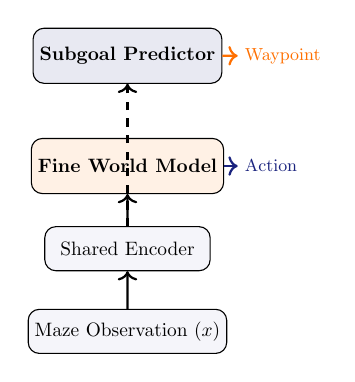
\begin{tikzpicture}[scale=0.7, every node/.style={scale=0.7}]
                \node[draw, rounded corners, fill=deepblue!10, minimum width=3cm, minimum height=1cm] (sg) at (0,2.5) {\textbf{Subgoal Predictor}};
                \node[draw, rounded corners, fill=accent!10, minimum width=3cm, minimum height=1cm] (wm) at (0,0.5) {\textbf{Fine World Model}};
                \node[draw, rounded corners, fill=lightbg, minimum width=3cm, minimum height=0.8cm] (enc) at (0,-1) {Shared Encoder};
                \node[draw, rounded corners, fill=lightbg, minimum width=3cm, minimum height=0.8cm] (maze) at (0,-2.5) {Maze Observation ($x$)};
                
                \draw[->, thick] (maze) -- (enc);
                \draw[->, thick] (enc) -- (wm);
                \draw[->, thick, dashed] (enc.north) -- ++(0,0.3) -| ($(sg.south)$);
                \draw[->, thick, accent] (sg) -- ++(2,0) node[right, text=accent] {\small Waypoint};
                \draw[->, thick, deepblue] (wm) -- ++(2,0) node[right, text=deepblue] {\small Action};
            \end{tikzpicture}
            \end{center}
        \end{column}
    \end{columns}
\end{frame}

\begin{frame}{The Problem: Catastrophic Forgetting}
    \textbf{Hypothesis:} Co-training both models should improve performance by learning a \textit{shared latent representation}.

    \vspace{0.4cm}
    \textbf{Reality:} The routing gradients from $\mathcal{L}_{\text{subgoal}}$ are orders of magnitude larger than the physics gradients from $\mathcal{L}_{\text{JEPA}}$.

    \vspace{0.3cm}
    \begin{alertblock}{Catastrophic Forgetting}
        During co-training, the massive routing gradients \textbf{overwrite} the encoder's learned physics representations. The agent forgets that walls are solid.
    \end{alertblock}

    \vspace{0.3cm}
    \begin{center}
        \textbf{Baseline:} 66\% $\longrightarrow$ \textbf{After naive co-training:} \textcolor{failred}{\textbf{6.25\%}} \quad (\textcolor{failred}{$\downarrow$59.75\%})
    \end{center}
\end{frame}

% ====================== SECTION 2 ======================
\section{Our Approach: Latent Distillation}

\begin{frame}{Latent Distillation: Core Idea}
    \textbf{Key insight:} Allow the encoder to adapt, but \textit{anchor} it to the proven physics manifold via a frozen reference.

    \vspace{0.3cm}
    \begin{center}
    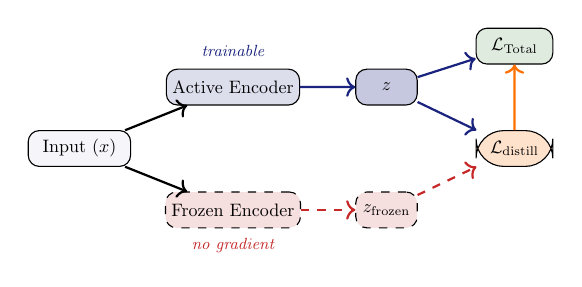
\begin{tikzpicture}[scale=0.65, every node/.style={scale=0.65, font=\normalsize}]
        % Input
        \node[draw, rounded corners, fill=lightbg, minimum width=2cm, minimum height=0.7cm] (input) at (0,0) {Input ($x$)};
        
        % Active path
        \node[draw, rounded corners, fill=deepblue!15, minimum width=2cm, minimum height=0.7cm] (active) at (3,1.2) {Active Encoder};
        \node[draw, rounded corners, fill=deepblue!25, minimum width=1.2cm, minimum height=0.7cm] (z) at (6,1.2) {$z$};
        
        % Frozen path
        \node[draw, rounded corners, fill=failred!15, minimum width=2cm, minimum height=0.7cm, dashed] (frozen) at (3,-1.2) {Frozen Encoder};
        \node[draw, rounded corners, fill=failred!15, minimum width=1.2cm, minimum height=0.7cm, dashed] (zf) at (6,-1.2) {$z_{\text{frozen}}$};
        
        % MSE
        \node[draw, rounded corners=10pt, fill=accent!20, minimum width=1.5cm, minimum height=0.7cm] (mse) at (8.5,0) {$\mathcal{L}_{\text{distill}}$};
        
        % Total Loss
        \node[draw, rounded corners, fill=successgreen!15, minimum width=1.5cm, minimum height=0.7cm] (loss) at (8.5,2) {$\mathcal{L}_{\text{Total}}$};
        
        % Arrows
        \draw[->, thick] (input) -- (active);
        \draw[->, thick] (input) -- (frozen);
        \draw[->, thick, deepblue] (active) -- (z);
        \draw[->, thick, failred, dashed] (frozen) -- (zf);
        \draw[->, thick, deepblue] (z) -- (mse);
        \draw[->, thick, failred, dashed] (zf) -- (mse);
        \draw[->, thick, accent] (mse) -- (loss);
        \draw[->, thick, deepblue] (z) -- (loss);
        
        % Labels
        \node[text=deepblue, font=\small\itshape] at (3,1.9) {trainable};
        \node[text=failred, font=\small\itshape] at (3,-1.9) {no gradient};
    \end{tikzpicture}
    \end{center}

    \vspace{0.2cm}
    The \textcolor{accent}{\textbf{MSE penalty}} acts as an \textit{elastic band}: the encoder can stretch to serve routing, but snaps back if it drifts too far from the physics baseline.
\end{frame}

\begin{frame}{Mathematical Formulation}
    \begin{block}{Total Loss Function}
    \vspace{0.2cm}
    $$ \mathcal{L}_{\text{Total}} = \underbrace{\mathcal{L}_{\text{JEPA}}}_{\text{physics}} + \lambda_{\text{aux}}\underbrace{\mathcal{L}_{\text{aux}}}_{\text{position}} + \lambda_{\text{sg}}\underbrace{\mathcal{L}_{\text{subgoal}}}_{\text{routing}} + \lambda_{\text{distill}} \cdot \underbrace{\text{MSE}(z,\, z_{\text{frozen}})}_{\textbf{our contribution}} $$
    \vspace{0.1cm}
    \end{block}

    \vspace{0.5cm}
    \textbf{Loss Components:}
    \begin{itemize}
        \item $\mathcal{L}_{\text{JEPA}}$: Prediction error on physical dynamics (walls, movement)
        \item $\mathcal{L}_{\text{aux}}$: Auxiliary $(x, y)$ position decoding from latent
        \item $\mathcal{L}_{\text{subgoal}}$: MSE to A*-optimal waypoint $N$ steps ahead
        \item $\textcolor{accent}{\text{MSE}(z, z_{\text{frozen}})}$: \textbf{Latent Distillation} --- keeps encoder on the physics manifold
    \end{itemize}
\end{frame}

\begin{frame}{Staged Unfreezing Strategy}
    \begin{center}
    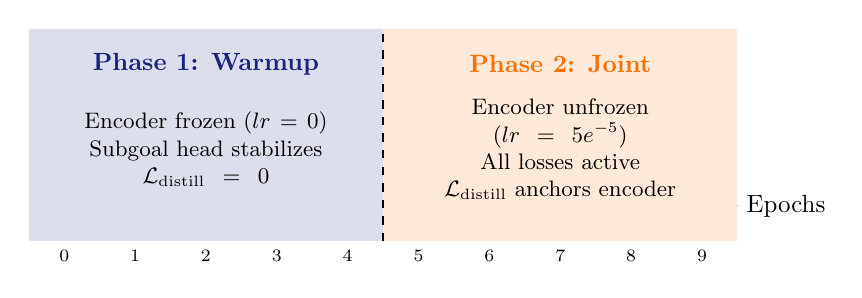
\begin{tikzpicture}[scale=0.9, every node/.style={scale=0.9}]
        % Timeline
        \draw[->, thick] (0,0) -- (10,0) node[right] {Epochs};
        
        % Phase 1
        \fill[deepblue!15] (0,-0.5) rectangle (5,2.5);
        \node[text=deepblue, font=\bfseries] at (2.5,2) {Phase 1: Warmup};
        \node[font=\small, text width=4cm, align=center] at (2.5,0.8) {Encoder frozen ($lr=0$)\\Subgoal head stabilizes\\$\mathcal{L}_{\text{distill}} = 0$};
        
        % Phase 2
        \fill[accent!15] (5,-0.5) rectangle (10,2.5);
        \node[text=accent, font=\bfseries] at (7.5,2) {Phase 2: Joint};
        \node[font=\small, text width=4cm, align=center] at (7.5,0.8) {Encoder unfrozen ($lr=5e^{-5}$)\\All losses active\\$\mathcal{L}_{\text{distill}}$ anchors encoder};
        
        % Divider
        \draw[thick, dashed] (5,-0.5) -- (5,2.5);
        
        % Epoch labels
        \foreach \x in {0,...,9} {
            \node[below, font=\scriptsize] at (\x+0.5, -0.5) {\x};
        }
    \end{tikzpicture}
    \end{center}

    \vspace{0.3cm}
    \textbf{Why staged?} At epoch 0 the subgoal head produces chaotic, random gradients. Unfreezing the encoder immediately would destroy the physics representations \textit{before} the distillation penalty can stabilize them.
\end{frame}

% ====================== SECTION 3 ======================
\section{Experimental Results}

\begin{frame}{Hyperparameter Sweep: $\lambda_{\text{distill}}$}
    \begin{table}[]
        \centering
        \renewcommand{\arraystretch}{1.3}
        \begin{tabular}{l c c c}
            \toprule
            \textbf{Strategy} & $\lambda_{\text{distill}}$ & \textbf{Success Rate} & \textbf{SPL} \\
            \midrule
            Frozen Baseline (no co-train) & --- & $\sim$66.00\% & $\sim$0.600 \\
            \textcolor{failred}{Naive Co-Training} & 0.0 & \textcolor{failred}{6.25\%} & \textcolor{failred}{0.059} \\
            \textcolor{failred}{Over-Distillation} & 50.0 & \textcolor{failred}{0.00\%} & \textcolor{failred}{0.000} \\
            \midrule
            \textcolor{successgreen}{\textbf{Latent Distillation (Ours)}} & \textbf{10.0} & \textcolor{successgreen}{\textbf{81.25\%}} & \textcolor{successgreen}{\textbf{0.751}} \\
            \bottomrule
        \end{tabular}
    \end{table}

    \vspace{0.4cm}
    \begin{itemize}
        \item $\lambda = 0$: No protection $\Rightarrow$ catastrophic forgetting (6.25\%).
        \item $\lambda = 50$: Too rigid $\Rightarrow$ encoder can't adapt at all (0\%).
        \item $\lambda = 10$: \textbf{Sweet spot} $\Rightarrow$ encoder adapts \textit{just enough} (\textbf{81.25\%}).
    \end{itemize}
\end{frame}

\begin{frame}{Visual Comparison: A*-Free Navigation}
    \begin{columns}[T]
        \begin{column}{0.48\textwidth}
            \begin{center}
                \textcolor{failred}{\textbf{Naive Co-Training ($\lambda=0$)}}\\[0.3cm]
                % Replace example-image-a with: figures/baseline_fail_unroll
                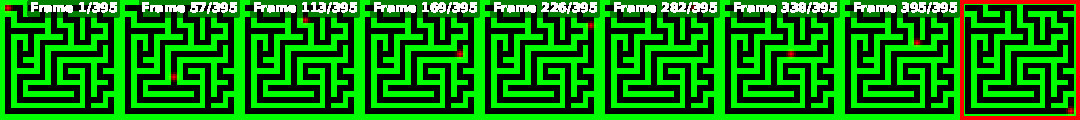
\includegraphics[width=\textwidth]{figures/baseline_fail_unroll}\\[0.2cm]
                {\small Agent crashes into walls repeatedly.\\Success: \textcolor{failred}{\textbf{6.25\%}}}
            \end{center}
        \end{column}
        \begin{column}{0.48\textwidth}
            \begin{center}
                \textcolor{successgreen}{\textbf{Latent Distillation ($\lambda=10$)}}\\[0.3cm]
                % Replace example-image-b with: figures/ours_success_unroll
                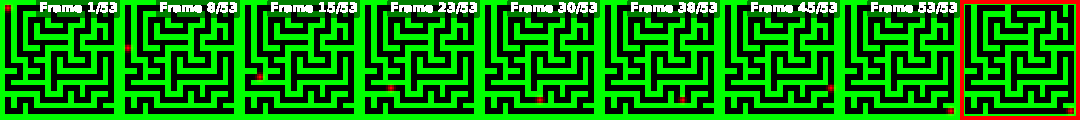
\includegraphics[width=\textwidth]{figures/ours_success_unroll}\\[0.2cm]
                {\small Agent navigates smoothly to the goal.\\Success: \textcolor{successgreen}{\textbf{81.25\%}}}
            \end{center}
        \end{column}
    \end{columns}
    
    \vspace{0.5cm}
    \begin{center}
        \small\textit{GIF animations available in \texttt{figures/} directory for live demo.}
    \end{center}
\end{frame}

\begin{frame}{Early Stopping: Why Epoch 4 is the Sweet Spot}
    \begin{center}
    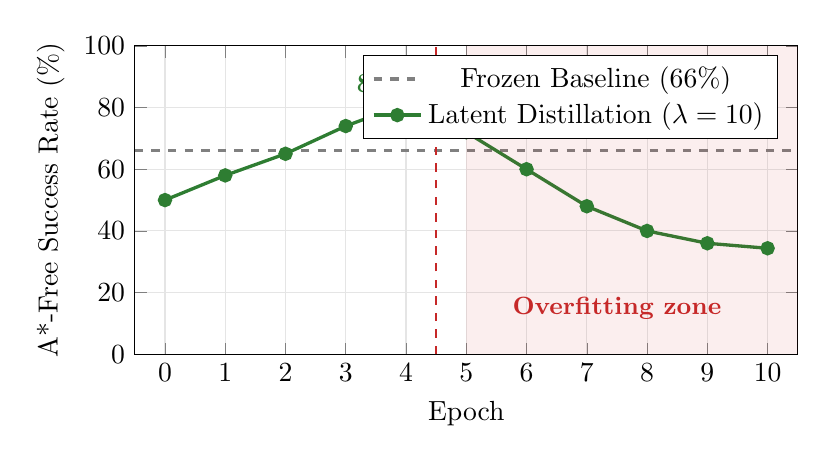
\begin{tikzpicture}
    \begin{axis}[
        width=10cm, height=5.5cm,
        xlabel={Epoch},
        ylabel={A*-Free Success Rate (\%)},
        xmin=-0.5, xmax=10.5,
        ymin=0, ymax=100,
        xtick={0,1,2,3,4,5,6,7,8,9,10},
        ytick={0,20,40,60,80,100},
        legend pos=north east,
        grid=major,
        grid style={gray!20},
        every axis plot/.append style={very thick},
    ]
    % Baseline reference line
    \addplot[dashed, gray, domain=-0.5:10.5] {66};
    \addlegendentry{Frozen Baseline (66\%)}

    % Our model curve (schematic based on eval data)
    \addplot[successgreen, mark=*, mark size=2pt] coordinates {
        (0,50) (1,58) (2,65) (3,74) (4,81.25) (5,72) (6,60) (7,48) (8,40) (9,36) (10,34.38)
    };
    \addlegendentry{Latent Distillation ($\lambda=10$)}

    % Peak annotation
    \node[anchor=south, text=successgreen, font=\bfseries] at (axis cs:4,81.25) {\textbf{81.25\%}};
    \draw[thick, failred, dashed] (axis cs:4.5,0) -- (axis cs:4.5,100);
    \node[anchor=south west, text=failred, font=\small\itshape] at (axis cs:4.6,85) {Encoder unfreezes};

    % Overfitting zone
    \fill[failred, opacity=0.08] (axis cs:5,0) rectangle (axis cs:10.5,100);
    \node[text=failred, font=\small\bfseries] at (axis cs:7.5,15) {Overfitting zone};

    \end{axis}
    \end{tikzpicture}
    \end{center}

    \vspace{0.2cm}
    \textbf{Key finding:} Performance peaks at the \textbf{end of warmup} (Epoch 4), then degrades as the unfrozen encoder gradually overfits to the routing loss. \textcolor{successgreen}{\textbf{Early stopping}} captures the optimal checkpoint.
\end{frame}

% ====================== SECTION 4 ======================
\section{Conclusion}

\begin{frame}{Conclusion \& Takeaways}
    \begin{enumerate}
        \item \textbf{Problem identified:} Naive co-training causes catastrophic forgetting (66\% $\to$ 6.25\%).
        \vspace{0.3cm}
        \item \textbf{Solution:} Latent Distillation via a frozen encoder reference and MSE penalty anchors the physics manifold during joint fine-tuning.
        \vspace{0.3cm}
        \item \textbf{Result:} \textcolor{successgreen}{\textbf{81.25\% A*-Free Success Rate}} --- an absolute \textbf{+15.25\%} improvement over the frozen baseline.
        \vspace{0.3cm}
        \item \textbf{Generalizable:} This technique applies to \textit{any} hierarchical model suffering from feature collapse during co-training.
    \end{enumerate}

    \vspace{0.8cm}
    \begin{center}
        \LARGE \textbf{Thank You --- Questions?}
    \end{center}
\end{frame}

\end{document}
